\chapter{Preliminary Analysis}\label{chap:preanalysis}
\section{Overview}
This chapter presents a preliminary analysis about JSMapper project. As a start, it includes an overview of how Linux kernel input subsystem works, how is the current state of joystick support under Linux, and how JSMapper approach fits into this schema to improve the situation.

\section{The Linux Kernel Input Subsystem}
The input subsystem is the part of the Linux kernel that manages, in a unified way, all the different input devices (such as keyboards, mouses, graphic tablets, joysticks, etc...) that can be attached to the system. It was designed with the clear goal in mind of hiding, almost completely from outside the kernel, the specific hardware interface (USB, PS/2, serial, etc....) the device was using to connect to the computer, while presenting an unique, consistent API interface to userspace that could easily be used by all the other system components that needed to deal with user input, like i.e. the console process or the X11 graphical window system.

The current Linux input subsystem is based mainly on the work of Vojtech Pavlik, who provided the initial implementation for a flexible joystick support API in 2.3 version, while also improving global USB support in the kernel. The work on the subject continued all along 2.4 and 2.5 versions, and finally in 2.6 the new, unified input subsystem fully replaced the old, hardware specifc support that previously existed on the kernel.

\subsection{Under the hood}
The input subsystem is mainly divided in three components, whose relationship is shown in the figure {\ref{fig:input_subsystem}} below:
\begin{itemize}
	\item the hardware drivers
	\item the input core
	\item the event handlers
\end{itemize}

\begin{figure}[htb]
\centering
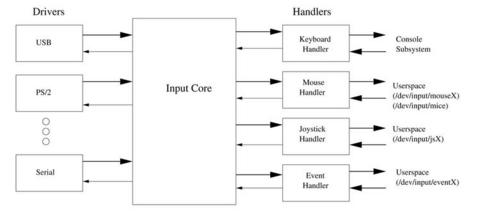
\includegraphics[width=0.8\textwidth]{input_subsystem}
\caption{The Linux kernel input subsystem architecture}
\label{fig:input_subsystem}
\end{figure}

These three elements of the input subsystem communicates each other by using \emph{events}, which are structures defined at kernel level containing all the information associated with a given input event, such as the button being pressed or released, its current state, the timestamp of the action, etc...

Note that, while most communication is done from hardware to drivers, from these to core, then to event filters and finally reaching to userspace, communication can also be done in the opposite way, this is, from userspace to hardware devices: this is how is possible i.e. to manipulate keyboard LED status, or to send i.e. motion commands to force-feedback capable driving wheels.

\subsection{Hardware drivers}
Hardware drivers are the part of the Linux input subsystem that directly interacts with the hardware. This is, there are a large number of available hardware device drivers. Most of them lay under the \emph{drivers/input} folder and subfolders of kernel source tree. There, they are organized either by bus type used to interact with the computer (\emph{gameport}, \emph{serio}, ...), or else by their device class type (such as \emph{joystick}, \emph{mouse}, \emph{keyboard}, ...).

Some other drivers lay into dedicated subtrees under Linux kernel. Among them, one of ther most important driver today for the input subsystem is the generic \emph{HID} driver (\emph{HID: Human Interface Device}), which implements support for the ``USB-HID'' specification. Effectively, most of the USB-based input devices available these days, including joysticks and similar, declare themselves as HID-compliant devices: this is a standard that provides an unified access model to the different elements conforming the device, such as buttons, keys, relative and absolute axes. 

By fully supporting HID-class specification, the number of supported input devices in Linux has raised dramatically, with dedicated hardware drivers being needed only for very specific tweaks.

In any case, the main function of any input subsystem hardware device driver is always the same: to deal with the specifics of the device and/or bus type, then generate an unified set of \emph{events} that will get injected into the input core, and later received by the event handlers attached to it.

\subsection{Input core}
The input core is the central part of the input subsystem, as it provides the needed communication between all the different components that conforms the input mechanism. 

Among the different tasks assigned to the input core, the main one of them is to receive the event notifications provided by the low-level hardware drivers, then route them to the different event handlers attached to the input core. The event handlers then can take the appropiate actions, which usually consist in some kind of notification to userspace.

Another one of the tasks performed by the input core is the responsability of notificating event handlers about new devices being plugged in (or removed from) the system, so event handlers can then decide if they must listen to the events provided by that particular device, or simply ignoring it. 

For instance, the existing \emph{joydev} module attaches to any joystick-type device attached, by querying if the device supports the specific subset of axes and key (button) ranges assigned to joystick devices. If so, then it creates a kernel device node (\emph{/dev/input/js0}, i.e.) that provides userspace with joystick API for that particular device.

\subsection{Event handlers}
Event handlers are basically at the receiving end of the kernel input subsystem architecture, and the final responsible of providing the userspace API for all other layers on the OS. Their role is to receive and dispatch the event notifications sent by the low-level hardware drivers of their interest, then provide an uniforn, consistent API to userspace for the device type they represent.

Effectively, every device handler provides a different API, which is intended to be useful for the particular type of device it represents. To do so, they register themselves as a ``handler'' inside the Linux kernel, which causes input core to notify them about any new (or existing) input device attached to the system: then, the event handler decides if such a device if of its interest (by inspecting some device flags) and, if so, creates a new device node (under \emph{/dev/input/}, usually, which provides the userspace API for that device.

These are some of input event handlers currently available in Linux kernel:
\begin{itemize}
	\item \emph{evdev}: generic input event handler. This is the primary input interface used by current Linux software layers (including X11 server, terminal emulators, etc..., and it's primarily used to get input events from both mouse and keyboards attached to the system.
	\item \emph{mousedev}: old mouse interface, mostly used to provide compatibility with old PS/2 mouse interface.
	\item \emph{keybdev}: also an old interface, this time used to provide compatibility with old VT keyboard API
	\item \emph{joydev}: joystick interface, providing existing Linux joystick API.
\end{itemize}

The way is designed, devices and event handlers are completely detached each other: this means, an event handler will simply provide a consistent input API to any device matching an specific set of characteristics, no matter how the device is actually built ot connected to the system. Also, the same device will sport more than one event handler, if it matches the characteristics required by more than one of them: for instance, a USB mouse / keyboard combo will feature two \emph{event} nodes (provided by the generic \emph{evdev} event handler), a \emph{mouse} node (provided for compatibility by the \emph{mousedev} handler), and maybe a \emph{kbd} node if the old \emph{keybdev} handler is loaded.

\subsubsection{Event filtering}
A very interesting feature of the event handlers (and of particular interest for JSMapper) is the possibility to register themselves as a \emph{``filter''} for the device, instead of as a regular handler: if so, then the input core will send any event first to \emph{filter}-type handlers, which has the possibility to filter out the event, and only after all filter-type handlers have dispatched the event (and only if none of them has blocked it), the event will reach the regular handler.

This is the method used by JSMapper to early intercept the events sent by the joystick device, and convert them to keyboard and mouse events without letting \emph{joydev} event handler to dispatch them.


\section{Joystick support on Linux}
As yet stated, current Linux support for joysticks is implemented by means of an special input event handler (\emph{joydev}),  which detects an provides a joystick-type API for any device plugged into the system featuring any of the following items:
\begin{itemize}
	\item An absolute axis identified either as ``X'', ``Wheel'', or ``Throttle''
	\item Any buttons whose IDs lay into into the range assigned for joysticks and gamepads
\end{itemize}

For such devices, the \emph{joydev} event handler will create a node (usually named \emph{/dev/input/js0} for the first device,\emph{/dev/input/js1} for the second and so on...), which userspace programs will use to access the joystick and take profit of it for games and so.

A typical sequence for a program using joystick support is to open the \emph{js} device created by \emph{joydev}, then using blocking \emph{read()} calls on it to read the \emph{``js\_event''} structures posted by the driver indicating the different events occurred. 
Listing~\ref{lst:joystick_api_sample} shows the typical workflow of a program using joystick API on Linux:
\lstinputlisting[language=C,
caption={Typical program flow for joystick Linux API},
label={lst:joystick_api_sample}]
{src/joystick_api_sample.c}

Alternatively, programs can use a more sophisticated approach by using \emph{select()} calls to detect when there is data (events) available for reading, or simply using the file handle in non-blocking mode, which will make the \emph{read()} call to return -1 in case there is no data available for reading.

In addition to the events returned by the \emph{read()} call, the API also features the following IOCTL control codes:
\begin{itemize}
	\item \textbf{JSIOCGVERSION}: returns API version
	\item \textbf{JSIOCGNAME}: returns device identifier string
	\item \textbf{JSIOCGBUTTONS}: returns number of buttons on the device
	\item \textbf{JSIOCGAXES}: returns number of axes on the device
	\item \textbf{JSIOCGCORR}, \textbf{JSIOCSCORR}: gets / sets axis correction values
	\item \textbf{JSIOCGAXMAP}, \textbf{JSIOCSAXMAP}: gets / sets axis mapping
	\item \textbf{JSIOCGBTNMAP}, \textbf{JSIOCSBTNMAP}: gets / sets button mapping
\end{itemize}

Listing~\ref{lst:joystick_api_ioctl_sample} shows an example of how IOCTL calls can be used to retrieve some device attributes:
\lstinputlisting[language=C,
caption={Using joystick IOCTL calls},
label={lst:joystick_api_ioctl_sample}]
{src/joystick_api_ioctl_sample.c}


\section{How JSMapper will work}
Based on this preliminary analysis, JSMapper will use the services provided by the input subsystem to achieve the desired functionality, which is the ability to intercept josytick events at a very low-level, then map then to simulated keyboard and mouse events, which will be programatically defined through a userspace API.

More specifically, JSMapper will be built as a kernel module (\emph{jsmapperdev}), which will behave in the following way:
\begin{itemize}
	\item it will declare itself as \emph{event handler} for joystick-alike devices, just as existing \emph{joydev} handler does, so it will get notified every time a device of such a type is plugged into the system.
	\item it will register explictly as a \emph{filter} for those devices, which will allow it to receive and intercept events \textbf{before} they reach the \emph{joydev} handler.
	\item it will use a \emph{virtual event generator} to generate and inject ``fake'' mouse and keyboard events into the input core, which will get routed in the usual upstream to userspace.
\end{itemize}

Also, for every joystick device attached to the system it will create a device node (\emph{/dev/input/jsmap0} for the first device, etc...), that will be the entry point for the programming API offered by the module. This API will allow external programs, such as the provided CLI tools, to program the device to map mouse and keyboard actions to the device elements, such as button and axes.


